\documentclass[11pt,a4paper]{article}

\usepackage[utf8]{inputenc}
\usepackage[margin=1in]{geometry}
\usepackage{amsmath,amssymb,amsfonts,amsthm}
\usepackage{algorithm}
\usepackage{algpseudocode}
\usepackage{tikz}
\usepackage{pgfplots}
\usepackage{booktabs}
\usepackage{multirow}
\usepackage{hyperref}
\usepackage{xcolor}
\usepackage{listings}
\usepackage{subcaption}
\usepackage{enumitem}

\usetikzlibrary{positioning,arrows.meta,shapes.geometric,fit,backgrounds}
\pgfplotsset{compat=1.18}

\newtheorem{theorem}{Theorem}[section]
\newtheorem{definition}[theorem]{Definition}

\newcommand{\keywords}[1]{\par\smallskip\noindent\textbf{Keywords:} #1}

\title{Post-Quantum Selective Disclosure for eIDAS~2.0 Credentials\\with Identity Escrow\\[0.5em]
\large A Transparent Hash-Based Construction from Sumcheck and Ligero}

\author{Oleksandr Vovkotrub\\
\small Independent Researcher\\
\small \texttt{alik@zk-eidas.com}}

\begin{document}
\maketitle

\begin{abstract}
The European Digital Identity framework (eIDAS~2.0) mandates digital identity
wallets for EU citizens, yet current credential presentation protocols reveal
more personal data than necessary. We present \textsc{zk-eidas}, a system for
privacy-preserving verification of ISO~18013-5 mdoc credentials using
zero-knowledge proofs from Sumcheck and Ligero. Our construction requires only
SHA-256---no bilinear pairings and no trusted setup---providing post-quantum
security for the proving system and offering a concrete migration path as
issuers adopt post-quantum signature schemes. We introduce an identity escrow
protocol combining ML-KEM-768 and AES-256-GCM that enables court-ordered
de-anonymization without breaking unlinkability, directly addressing eIDAS
accountability requirements. Our predicate system supports equality, comparison,
range, set membership, and Boolean composition over credential claims. We
demonstrate \textasciitilde17\,ms ECDSA signature verification within the
circuit, with end-to-end proving under 200\,ms for multi-attribute credentials.
We provide comprehensive benchmarks and map our construction to EUDI
Architecture Reference Framework requirements.
\end{abstract}

\keywords{zero-knowledge proofs \and selective disclosure \and eIDAS~2.0
\and post-quantum cryptography \and identity escrow \and anonymous credentials}

\section{Introduction}\label{sec:intro}
% Content to be written

\section{Background and Preliminaries}\label{sec:background}
% Content to be written

% !TEX root = ../main.tex
\section{Construction}\label{sec:construction}

We now present the \textsc{zk-eidas} construction in full.
Section~\ref{sec:model} defines the system model, roles, and security properties.
Section~\ref{sec:parsing} describes the credential parsing circuit that ingests raw mdoc CBOR bytes and produces a zero-knowledge proof.
Section~\ref{sec:predicates} formalises the predicate system used for selective disclosure.
Section~\ref{sec:nullifiers} specifies nullifiers and holder binding.

%% ───────────────────────────────────────────────────────────────────
\subsection{System Model and Definitions}\label{sec:model}

\paragraph{Roles.}
The construction involves four parties:
\begin{itemize}
  \item \textbf{Issuer $\mathcal{I}$}. Issues mobile driving licence (mdoc) credentials conforming to ISO/IEC~18013-5~\cite{iso18013}. The issuer signs the Mobile Security Object (MSO) with ECDSA over the NIST~P-256 curve. Our construction requires \emph{no modifications} to the issuer.
  \item \textbf{Holder $\mathcal{H}$}. Possesses an mdoc credential and generates zero-knowledge proofs of predicate satisfaction. The holder runs the proving algorithm on their device.
  \item \textbf{Verifier $\mathcal{V}$}. Receives a proof and verifies it. The verifier learns only the Boolean result of each requested predicate --- no attribute values are revealed.
  \item \textbf{Escrow Authority $\mathcal{E}$}. Holds an ML-KEM-768 decapsulation key~\cite{fips203}. The authority can decrypt the holder's escrowed identity fields only when presented with a valid court order or arbitration ruling.
\end{itemize}

\paragraph{Security properties.}
We require the following properties, stated semi-formally below.

\begin{definition}[Completeness]\label{def:completeness}
  For every honestly issued credential $C$, set of predicates $\{P_i\}$ that $C$ satisfies, and honestly generated escrow ciphertext, the proof produced by an honest holder is accepted by the verifier with probability~$1$.
\end{definition}

\begin{definition}[Soundness]\label{def:soundness}
  For any probabilistic polynomial-time adversary $\mathcal{A}$, the probability that $\mathcal{A}$ produces a proof $\pi$ that is accepted by the verifier for a statement $x \notin \mathcal{L}$ is bounded by a negligible function $\mathsf{negl}(\lambda)$:
  \[
    \Pr\bigl[\mathsf{Verify}(\mathsf{vk}, x, \pi) = 1 \;\wedge\; x \notin \mathcal{L}\bigr] \leq \mathsf{negl}(\lambda).
  \]
  In our setting, $x \notin \mathcal{L}$ means either the credential signature is invalid, or at least one predicate is not satisfied by the actual attribute value.
\end{definition}

\begin{definition}[Zero-Knowledge]\label{def:zk}
  There exists a probabilistic polynomial-time simulator $\mathcal{S}$ such that for every verifier $\mathcal{V}^*$, the view of $\mathcal{V}^*$ when interacting with an honest prover on witness $w$ is computationally indistinguishable from the output of $\mathcal{S}(x)$ given only the statement:
  \[
    \bigl\{\mathsf{View}_{\mathcal{V}^*}(\mathcal{H}(w) \leftrightarrow \mathcal{V}^*)\bigr\}
    \;\approx_c\;
    \bigl\{\mathcal{S}(x)\bigr\}.
  \]
  In particular, $\mathcal{V}^*$ learns nothing about the credential beyond the truth value of the requested predicates.
\end{definition}

\begin{definition}[Unlinkability]\label{def:unlinkability}
  Let $\pi_0$ and $\pi_1$ be two proofs generated by the same holder from the same credential under different verifier scopes (i.e., distinct contract hashes $c_0 \neq c_1$). No probabilistic polynomial-time distinguisher $\mathcal{D}$ can determine whether $\pi_0$ and $\pi_1$ originate from the same credential with advantage greater than $\mathsf{negl}(\lambda)$.
\end{definition}

\begin{definition}[Escrow Correctness]\label{def:escrow-correct}
  If the holder honestly encrypts identity fields $\{f_i\}$ under the authority's ML-KEM-768 public key, then the authority recovers $\{f_i\}$ exactly upon decapsulation and AES-256-GCM decryption.
\end{definition}

\begin{definition}[Non-Frameability]\label{def:non-frame}
  No coalition of a malicious authority $\mathcal{E}^*$ and a malicious verifier $\mathcal{V}^*$ can produce a valid escrow ciphertext that, when decrypted, yields identity fields belonging to an honest holder $\mathcal{H}$ who did not participate in the protocol, except with probability $\mathsf{negl}(\lambda)$.
\end{definition}

\paragraph{Threat model.}
We consider the following adversarial capabilities:
\begin{itemize}
  \item \emph{Verifiers} are honest-but-curious: they follow the protocol but attempt to extract information from transcripts.
  \item \emph{Holders} are potentially malicious: they may attempt to prove false statements or use forged credentials.
  \item \emph{The escrow authority} is honest-but-curious: it holds the decapsulation key faithfully but may attempt to learn holder identities from escrowed data without authorisation.
  \item \emph{Collusion}: even if a verifier and the escrow authority collude, they cannot break unlinkability (Definition~\ref{def:unlinkability}) without a court order that triggers decapsulation. The scoped nullifier mechanism ensures that the authority sees only an encrypted blob, and the verifier sees only a nullifier hash --- neither alone nor together suffices to link presentations across different scopes.
  \item \emph{Issuers} are assumed honest. A malicious or compromised issuer could craft credentials with colliding digests in the MSO or embed subliminal information in the ECDSA signature nonce. These attacks are outside our scope: mitigating them requires issuer-side controls (e.g., deterministic ECDSA nonces per RFC~6979) rather than proving-system changes.
\end{itemize}

%% ───────────────────────────────────────────────────────────────────
\subsection{Credential Parsing Circuit}\label{sec:parsing}

The core contribution of \textsc{zk-eidas} is a \emph{monolithic} Longfellow circuit~\cite{longfellow} that ingests raw mdoc CBOR bytes and performs all verification steps --- CBOR parsing, digest chain validation, ECDSA P-256 signature verification, predicate evaluation, nullifier derivation, and escrow digest computation --- within a single proof.  No trusted preprocessing step transforms the credential before it enters the circuit.

Algorithm~\ref{alg:prove} presents the proving procedure.

\begin{algorithm}[t]
  \caption{$\mathsf{Prove}$: mdoc selective-disclosure proof generation}\label{alg:prove}
  \begin{algorithmic}[1]
    \Require mdoc bytes $m$; issuer public key $\mathit{pk} = (x,y) \in \mathbb{F}_p^2$ (P-256); session transcript $\mathit{st}$; requested attributes $\{(ns_i, id_i, v_i, t_i)\}_{i=1}^{k}$; current time $\mathit{now}$; contract hash $c \in \{0,1\}^{64}$; escrow fields $\{e_j\}_{j=0}^{7} \subset \{0,1\}^{256}$
    \Ensure proof bytes $\pi$; nullifier hash $\eta$; binding hash $\beta$; escrow digest $\delta$
    \Statex
    \State Parse CBOR structure from $m$
      \Comment{in-circuit CBOR decoder}
    \State Extract $\mathsf{IssuerAuth}$ (COSE\_Sign1 envelope) from $m$
    \State Extract MSO $\gets$ payload of $\mathsf{IssuerAuth}$
    \For{each requested attribute $(ns_i, id_i, v_i, t_i)$}
      \State Locate $\mathsf{IssuerSignedItem}$ for $(ns_i, id_i)$ in the CBOR structure
      \State $d_i \gets \mathsf{SHA\textnormal{-}256}(\mathsf{IssuerSignedItem})$
      \State \textbf{assert} $d_i = \mathsf{MSO.valueDigests}[ns_i][\mathsf{digestID}]$
        \Comment{digest chain}
      \State $v'_i \gets$ extract $\mathsf{elementValue}$ from CBOR encoding
      \State Evaluate predicate $(v'_i, v_i, t_i)$
        \Comment{see \S\ref{sec:predicates}}
    \EndFor
    \State Verify $\mathsf{ECDSA}_{pk}$ signature on $\mathsf{IssuerAuth}$
      \Comment{P-256, see below}
    \State $\eta \gets \mathsf{SHA\textnormal{-}256}(m \,\|\, c)$
      \Comment{scoped nullifier}
    \State $\beta \gets \mathsf{SHA\textnormal{-}256}(\mathsf{attr}_0[0..31])$
      \Comment{holder binding}
    \State $\delta \gets \mathsf{SHA\textnormal{-}256}(e_0 \,\|\, e_1 \,\|\, \cdots \,\|\, e_7)$
      \Comment{escrow digest}
    \State \Return $(\pi, \eta, \beta, \delta)$
  \end{algorithmic}
\end{algorithm}

\paragraph{Single-circuit architecture.}
A critical design choice is that all steps 1--14 of Algorithm~\ref{alg:prove} execute inside a \emph{single} Longfellow circuit instance.  The circuit takes raw CBOR bytes as private input and produces $({\eta}, {\beta}, {\delta})$ as public outputs.  The Sumcheck+Ligero proof system~\cite{sumcheck,ligero} then proves knowledge of a satisfying assignment.  This monolithic approach eliminates the need for intermediate commitments or multi-circuit composition, keeping the critical path shallow (circuit depth~22 for the signature sub-circuit, depth~21 for the hash sub-circuit).

\paragraph{Circuit topology.}
Longfellow compiles the circuit into two sub-circuits that are composed internally:
\begin{enumerate}
  \item A \emph{hash sub-circuit} over $\mathsf{GF}(2^{128})$ containing ${\sim}\,4 \times 10^6$ wires and ${\sim}\,99{,}000$ public inputs.  This sub-circuit handles CBOR parsing, SHA-256 digest chain verification, predicate evaluation, nullifier computation, binding hash, and escrow digest.
  \item A \emph{signature sub-circuit} over $\mathsf{GF}(2^{128})$ containing ${\sim}\,224{,}000$ wires and ${\sim}\,3{,}700$ public inputs.  This sub-circuit handles ECDSA~P-256 signature verification.
\end{enumerate}
The two sub-circuits are proven independently (each via Sumcheck+Ligero) and their proofs are concatenated.  Shared values between sub-circuits are committed to in both proofs.

\paragraph{ECDSA in-circuit.}
P-256 signature verification is the most expensive component, requiring ${\sim}\,17\,\text{ms}$ of the ${\sim}\,280\,\text{ms}$ proving time for the signature sub-circuit.  Working over $\mathsf{GF}(2^{128})$ provides efficient native SHA-256 gates, but ECDSA requires field arithmetic over $\mathbb{F}_p$ where $p$ is the P-256 prime.  We handle this via \emph{range-checked limb decomposition}: each 256-bit P-256 field element is decomposed into limbs that fit within the $\mathsf{GF}(2^{128})$ arithmetic, with range checks ensuring no overflow.  Scalar multiplication is performed using a double-and-add circuit with constant-time conditional moves.

%% ───────────────────────────────────────────────────────────────────
\subsection{Predicate System}\label{sec:predicates}

Each attribute carries a \emph{verification type} $t \in \{0,1,2,3\}$ that determines which predicate the circuit enforces on the attribute value.  Table~\ref{tab:predicates} lists the four primitive types.

\begin{table}[t]
  \centering
  \caption{Primitive predicate types.  Here $v$ is the actual attribute value extracted from the credential, and $v'$ is the expected value supplied by the verifier.}\label{tab:predicates}
  \begin{tabular}{clll}
    \toprule
    Code & Type & Constraint & Semantics \\
    \midrule
    0 & Equality      & $v = v'$    & Value matches exactly \\
    1 & Less-or-equal & $v \leq v'$ & Value at most $v'$ \\
    2 & Greater-or-equal & $v \geq v'$ & Value at least $v'$ \\
    3 & Not-equal     & $v \neq v'$ & Value differs from $v'$ \\
    \bottomrule
  \end{tabular}
\end{table}

\paragraph{In-circuit comparison.}
Algorithm~\ref{alg:predicate} describes how the circuit evaluates a predicate.  All comparisons are \emph{lexicographic} over the byte-level representation, using a binary comparator sub-circuit.

\begin{algorithm}[t]
  \caption{$\mathsf{EvalPredicate}$: in-circuit predicate evaluation}\label{alg:predicate}
  \begin{algorithmic}[1]
    \Require Actual value $v \in \{0,1\}^n$; expected value $v' \in \{0,1\}^n$; type $t \in \{0,1,2,3\}$
    \Ensure Assertion that the predicate holds
    \Statex
    \State $\mathit{is\_leq} \gets \mathsf{CMP.leq}(n,\, v,\, v')$
      \Comment{$1$ iff $v \leq v'$ lexicographically}
    \State $\mathit{is\_geq} \gets \mathsf{CMP.leq}(n,\, v',\, v)$
      \Comment{$1$ iff $v' \leq v$, i.e.\ $v \geq v'$}
    \State $\mathit{is\_eq} \gets \mathit{is\_leq} \wedge \mathit{is\_geq}$
      \Comment{$v = v'$ iff both hold}
    \State $\mathit{pass} \gets \mathsf{MUX}\bigl(t,\; \mathit{is\_eq},\; \mathit{is\_leq},\; \mathit{is\_geq},\; \neg\,\mathit{is\_eq}\bigr)$
    \State \textbf{assert} $\mathit{pass} = 1$
  \end{algorithmic}
\end{algorithm}

The multiplexer $\mathsf{MUX}$ selects the appropriate Boolean based on the type code~$t$: equality ($t=0$) checks $\mathit{is\_eq}$; less-or-equal ($t=1$) checks $\mathit{is\_leq}$; greater-or-equal ($t=2$) checks $\mathit{is\_geq}$; not-equal ($t=3$) checks $\neg\,\mathit{is\_eq}$.  The assertion is enforced as a hard constraint --- if it fails, the circuit is unsatisfiable and no valid proof can be produced.

\paragraph{Composed predicates.}
While the circuit supports only the four primitive types, the API layer composes them into richer predicates before circuit entry:
\begin{itemize}
  \item \textbf{Range} $[\ell, h]$: decomposed into two attribute requests on the same claim --- one with type $\mathsf{GEQ}(\ell)$ and one with type $\mathsf{LEQ}(h)$.  Both must pass for the proof to succeed.
  \item \textbf{Set membership} $\{v_1, \ldots, v_k\}$: decomposed into $k$ attribute requests with type $\mathsf{EQ}$, combined with a logical~OR at the API layer (at least one must match).  The cost is linear in~$k$: each element adds one attribute slot to the circuit.  For small sets (e.g., EU nationality among 27~Member States) this is practical; for large sets, a Merkle-based membership proof would amortise the cost to $O(\log k)$ and is a natural extension.
  \item \textbf{Boolean combinators}: arbitrary $\mathsf{AND}$ and $\mathsf{OR}$ trees over sub-predicates, resolved by the facade before generating the attribute list passed to the circuit.
\end{itemize}

\paragraph{Date handling.}
CBOR-encoded date attributes in mdoc credentials use the ISO~8601 \emph{full-date} profile (\texttt{YYYY-MM-DD}), e.g., \texttt{"1998-09-04"}.  A key observation is that strings in this fixed-width format sort correctly under lexicographic comparison: for dates $d_1 < d_2$ in calendar order, the byte representation satisfies $d_1 <_{\mathrm{lex}} d_2$.  (This property does \emph{not} hold for arbitrary ISO~8601 representations that include time-zone offsets.)  This allows the circuit to perform date comparisons (e.g., ``birth date $\leq$ cutoff date'' for age proofs) using the same $\mathsf{CMP.leq}$ comparator used for all other predicates, without requiring epoch conversion or calendar arithmetic inside the circuit.

%% ───────────────────────────────────────────────────────────────────
\subsection{Nullifiers and Holder Binding}\label{sec:nullifiers}

\paragraph{Scoped nullifiers.}
To enable double-use detection without sacrificing cross-service unlinkability, we employ \emph{scoped nullifiers}.  The nullifier is computed inside the hash sub-circuit as:
\[
  \eta \;=\; \mathsf{SHA\textnormal{-}256}\bigl(m \,\|\, c\bigr),
\]
where $m$ is the raw mdoc CBOR byte string (private input) and $c \in \{0,1\}^{64}$ is a verifier-chosen \emph{contract hash} (public input).  The contract hash serves as a domain separator --- for instance, the SHA-256 hash of the service URL or a session identifier.

This construction satisfies two properties simultaneously:
\begin{enumerate}
  \item \textbf{Replay detection within scope.}  Presenting the same credential to the same verifier (same~$c$) produces the same nullifier~$\eta$.  The verifier maintains a set of seen nullifiers and rejects duplicates.
  \item \textbf{Unlinkability across scopes.}  Presenting the same credential to two different verifiers (distinct $c_0 \neq c_1$) produces distinct nullifiers $\eta_0 \neq \eta_1$.  Since SHA-256 is modelled as a random oracle, no efficient adversary can determine whether $\eta_0$ and $\eta_1$ originate from the same credential, satisfying Definition~\ref{def:unlinkability}.
\end{enumerate}

\paragraph{Threat-model limitation.}
Because the nullifier is a deterministic function of the credential bytes~$m$ (not of a holder-held secret), an adversary who obtains~$m$ --- for instance, from a compromised device --- can compute $\eta = \mathsf{SHA\textnormal{-}256}(m \| c)$ for any scope~$c$ and check whether a published nullifier corresponds to that credential.  This is weaker than systems where nullifiers derive from a secret key held by the holder.  Incorporating a holder secret into the nullifier would require an additional private input to the circuit and a corresponding key-management protocol; we leave this extension to future work.

\paragraph{Holder binding.}
In addition to the nullifier, the circuit computes a \emph{binding hash}:
\[
  \beta \;=\; \mathsf{SHA\textnormal{-}256}\bigl(\mathsf{attr}_0[0..31]\bigr),
\]
where $\mathsf{attr}_0[0..31]$ denotes the first 32~bytes of the first requested attribute's CBOR-encoded value.  In practice, the holder controls which attribute appears first by choosing the order of the attribute request list; for cross-credential linking, the holder should place the same claim (e.g., the PID unique identifier) first in both requests.  If two credentials from different issuers happen to share the same first attribute value, the binding hashes will collide --- this is an inherent property of binding to a claim value rather than to a holder secret, and mirrors the nullifier limitation discussed above.

The binding hash serves two purposes:
\begin{enumerate}
  \item It binds the proof to a specific holder identity without revealing \emph{which} attribute was used, since $\beta$ is a one-way hash.
  \item It enables \emph{opt-in cross-credential linking}: if a holder presents two different credentials (e.g., a driving licence and a health insurance card) that share the same first attribute value, the binding hashes will match, allowing a verifier to confirm that both credentials belong to the same person --- but only if the holder chooses to present them.
\end{enumerate}

Both $\eta$ and $\beta$ are computed inside the hash sub-circuit as part of its single evaluation pass, adding only two SHA-256 invocations (each a chain of compression calls) to the existing circuit.

\paragraph{Design rationale.}
Some zero-knowledge credential systems (e.g., those based on CL-signatures~\cite{camenisch2001}) compose multiple sub-protocols via MAC chains or commitment-and-prove techniques, which increases the circuit depth or requires interactive rounds.  In \textsc{zk-eidas}, the nullifier, binding hash, and escrow digest are all computed within the \emph{same} Longfellow circuit that verifies the credential.  This single-circuit approach keeps the critical path short (depth~21 for the hash sub-circuit) and avoids the need for cross-proof consistency checks, reducing both proving time and implementation complexity.

% !TEX root = ../main.tex
\section{Identity Escrow Protocol}\label{sec:escrow}

Zero-knowledge credential systems face a fundamental tension:
privacy requires that presentations reveal nothing beyond the truth
value of the requested predicates, yet the rule of law demands that,
under judicial authorisation, the identity behind a fraudulent or
harmful transaction can be recovered.
This section presents the \textsc{zk-eidas} identity escrow protocol,
which resolves this tension by encrypting identifying fields
\emph{per presentation} under a designated escrow authority's
post-quantum public key, with an in-circuit binding that
prevents substitution of the encrypted payload.

%% ───────────────────────────────────────────────────────────────────
\subsection{Motivation and Regulatory Requirement}\label{sec:escrow-motivation}

Article~5a of the eIDAS~2.0 Regulation requires that member states
ensure the possibility of identifying natural persons behind
electronic transactions when mandated by a court order or other
legitimate judicial authorisation.  An anonymous credential system
that provides \emph{no} mechanism for accountability creates a legal
vacuum: it cannot be deployed in any eIDAS-regulated context, because
no lawful process exists to trace a fraudulent presentation back to
its holder.

\paragraph{Existing approaches and their limitations.}
The literature offers several mechanisms for revocable anonymity, each
with significant drawbacks in the eIDAS setting:

\begin{itemize}
  \item \textbf{Group signatures}~\cite{camenisch2001}.
    A group manager can open \emph{any} signature produced by any group
    member, creating a single point of failure.  If the group manager is
    compromised, every past and future presentation is deanonymisable.
    Moreover, the opening power is unconditional --- it is not
    scoped to a court order or a specific presentation.

  \item \textbf{Trusted third parties (online escrow).}
    Some designs require the holder to contact an online escrow agent
    at each presentation to obtain a blinded token.  This introduces an
    availability risk (the escrow agent becomes a service bottleneck)
    and a correlation risk (the agent learns the timing and frequency
    of presentations, even if it does not learn the content).

  \item \textbf{Revocable anonymity via accumulators.}
    Accumulator-based revocation schemes~\cite{camenisch2001} are
    designed for credential \emph{revocation} (removing a holder from
    the valid set), not for per-presentation accountability.  They do
    not provide a mechanism to recover the identity behind a specific
    transaction; they can only exclude a known holder from future
    transactions.
\end{itemize}

\paragraph{Our approach.}
We adopt a \emph{per-presentation encryption} strategy.  At each
proof generation, the holder encrypts a configurable set of
identifying fields (e.g., name and date of birth) under the escrow
authority's ML-KEM-768 encapsulation key~\cite{fips203}.  The
resulting ciphertext is bound to the zero-knowledge proof via an
in-circuit SHA-256 digest, so that the verifier can later confirm ---
after a court-ordered decryption --- that the recovered identity
matches the proof.  Crucially:
\begin{enumerate}
  \item Each presentation uses a \emph{fresh} ML-KEM encapsulation,
    so ciphertexts from different presentations are unlinkable
    (Theorem~\ref{thm:unlinkability}).
  \item The escrow authority holds only a decapsulation key; it cannot
    decrypt without possessing the per-presentation ciphertext, and it
    learns nothing from observing the proof itself.
  \item No online interaction with the authority is required at
    presentation time.
\end{enumerate}

%% ───────────────────────────────────────────────────────────────────
\subsection{Construction}\label{sec:escrow-construction}

We describe the escrow protocol as four procedures:
$\mathsf{KeyGen}$ (authority setup),
$\mathsf{Escrow}$ (holder encryption during proof generation),
$\mathsf{Bind}$ (in-circuit digest computation), and
$\mathsf{Recover}$ (authority decryption upon court order).

\medskip

\begin{algorithm}[t]
  \caption{$\mathcal{E}.\mathsf{KeyGen}$: Escrow authority key generation}\label{alg:keygen}
  \begin{algorithmic}[1]
    \Ensure Encapsulation key $\mathit{ek}$; seed $s$
    \Statex
    \State $s \gets\!\!\!\!\$\ \{0,1\}^{512}$
      \Comment{64-byte random seed}
    \State $\mathit{dk} \gets \textsf{ML-KEM-768}.\mathsf{DeriveKey}(s)$
      \Comment{FIPS 203~\cite{fips203}}
    \State $\mathit{ek} \gets \mathit{dk}.\mathsf{EncapsulationKey}()$
      \Comment{1184 bytes}
    \State Publish $\mathit{ek}$
    \State Store $s$ securely
      \Comment{offline, hardware-protected}
    \State \Return $(\mathit{ek}, s)$
  \end{algorithmic}
\end{algorithm}

\begin{algorithm}[t]
  \caption{$\mathcal{H}.\mathsf{Escrow}$: Per-presentation field encryption (holder side)}\label{alg:escrow}
  \begin{algorithmic}[1]
    \Require Field values $\{f_i\}_{i=0}^{n-1}$ ($n \leq 8$, each a byte string); encapsulation key $\mathit{ek}$
    \Ensure Envelope $\mathcal{E}\mathit{nv} = (\mathit{cts}[], \mathit{tags}[], \mathit{ek\_blob}, \mathit{names}[])$
    \Statex
    \State $K \gets\!\!\!\!\$\ \{0,1\}^{248}$
      \Comment{31-byte symmetric key, zero-padded to 32 bytes}
    \For{$i = 0, \ldots, n-1$}
      \State $\mathit{nonce}_i \gets 0^{64} \,\|\, i$
        \Comment{12-byte nonce, counter mode}
      \State $(\mathit{ct}_i, \mathit{tag}_i) \gets \textsf{AES-256-GCM}.\mathsf{Enc}(K, \mathit{nonce}_i, f_i)$
    \EndFor
    \State $(c, \mathit{ss}) \gets \textsf{ML-KEM-768}.\mathsf{Encaps}(\mathit{ek})$
      \Comment{$c$: 1088 bytes}
    \State $\mathit{mask} \gets \mathsf{SHA\textnormal{-}256}(\mathit{ss})$
      \Comment{32-byte mask}
    \State $\mathit{enc}_K \gets K \oplus \mathit{mask}$
      \Comment{32 bytes}
    \State \Return $\bigl(\{\mathit{ct}_i\}, \{\mathit{tag}_i\}, c \,\|\, \mathit{enc}_K, \{\mathit{name}_i\}\bigr)$
  \end{algorithmic}
\end{algorithm}

\begin{algorithm}[t]
  \caption{$\mathsf{Bind}$: In-circuit escrow digest (inside Longfellow hash sub-circuit)}\label{alg:bind}
  \begin{algorithmic}[1]
    \Require Escrow field values $\{e_j\}_{j=0}^{7}$, each $\in \{0,1\}^{256}$ (32-byte zero-padded claim values)
    \Ensure Public output $\delta$ (escrow digest)
    \Statex
    \State $\delta \gets \mathsf{SHA\textnormal{-}256}(e_0 \,\|\, e_1 \,\|\, \cdots \,\|\, e_7)$
      \Comment{256-byte input, single hash}
    \State \textbf{output} $\delta$ as public
  \end{algorithmic}
\end{algorithm}

Algorithm~\ref{alg:bind} is executed within the same Longfellow circuit~\cite{longfellow} that verifies the credential (Algorithm~\ref{alg:prove}).  The escrow digest~$\delta$ appears as a public output alongside the nullifier~$\eta$ and binding hash~$\beta$.  Because the circuit takes the raw claim values as private input and hashes them deterministically, the digest commits to the \emph{actual} credential fields --- not to values chosen by the holder after the fact.

The verifier receives the proof (containing~$\delta$) and the envelope produced by Algorithm~\ref{alg:escrow}.  It stores both.  The binding is verified \emph{only after court-ordered decryption}: the authority decrypts the envelope, pads each recovered field to 32~bytes, computes $\mathsf{SHA\textnormal{-}256}(e_0 \| \cdots \| e_7)$, and checks equality with~$\delta$.  A mismatch indicates tampering.

\begin{algorithm}[t]
  \caption{$\mathcal{E}.\mathsf{Recover}$: Identity recovery upon court order}\label{alg:recover}
  \begin{algorithmic}[1]
    \Require Envelope $\mathcal{E}\mathit{nv}$; authority seed $s$
    \Ensure Plaintext fields $\{f_i\}_{i=0}^{n-1}$
    \Statex
    \State $\mathit{dk} \gets \textsf{ML-KEM-768}.\mathsf{DeriveKey}(s)$
    \State Parse $c \,\|\, \mathit{enc}_K$ from $\mathcal{E}\mathit{nv}.\mathit{ek\_blob}$
    \State $\mathit{ss} \gets \textsf{ML-KEM-768}.\mathsf{Decaps}(\mathit{dk}, c)$
    \State $\mathit{mask} \gets \mathsf{SHA\textnormal{-}256}(\mathit{ss})$
    \State $K \gets \mathit{enc}_K \oplus \mathit{mask}$
    \For{$i = 0, \ldots, n-1$}
      \State $\mathit{nonce}_i \gets 0^{64} \,\|\, i$
      \State $f_i \gets \textsf{AES-256-GCM}.\mathsf{Dec}(K, \mathit{nonce}_i, \mathit{ct}_i \,\|\, \mathit{tag}_i)$
    \EndFor
    \State \Return $\{f_i\}_{i=0}^{n-1}$
  \end{algorithmic}
\end{algorithm}

\paragraph{Concrete sizes.}
For a typical escrow envelope containing two fields (family name and date of birth), the overhead is dominated by the ML-KEM-768 ciphertext: $1088 + 32 = 1120$~bytes for the key blob, plus approximately $2 \times (32 + 16) = 96$~bytes for the AES-256-GCM ciphertexts and tags, totalling roughly 1.2~KB.  This is appended to the proof, which itself is approximately 365~KB (see Section~\ref{sec:benchmarks}).

\begin{figure}[t]
\centering
% !TEX root = ../main.tex
% Figure: Identity escrow protocol sequence diagram
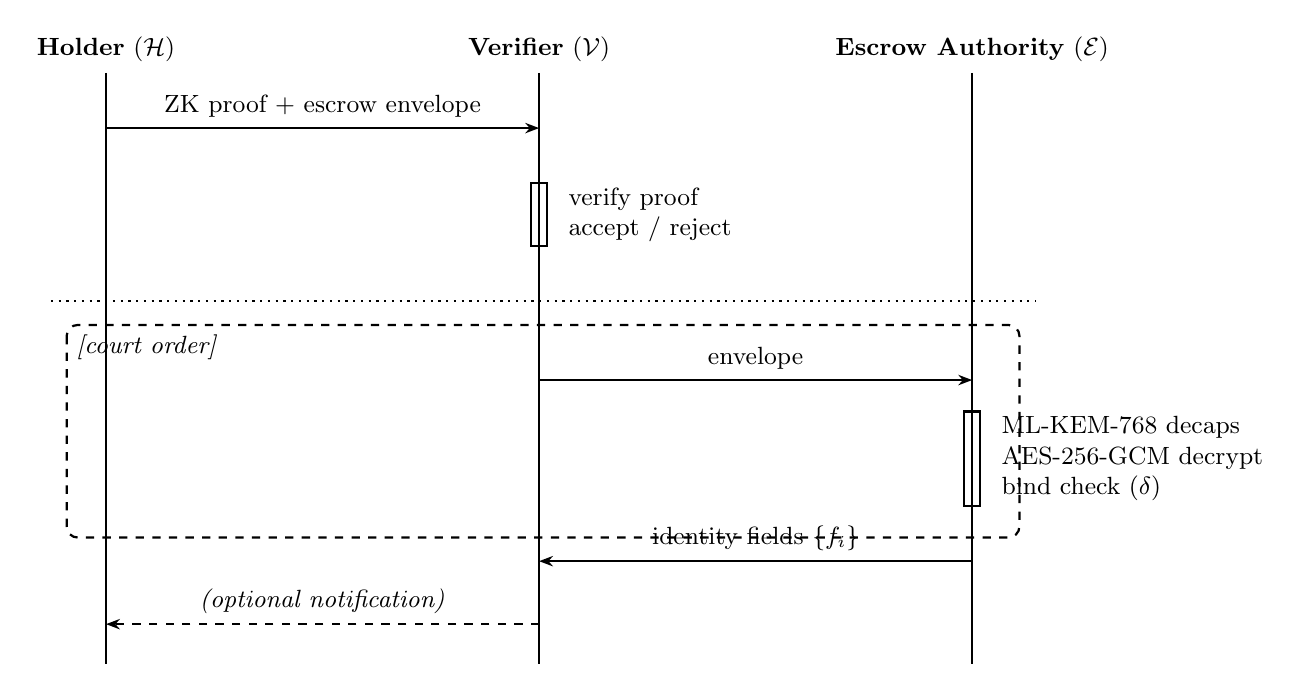
\begin{tikzpicture}[
  node distance=0 and 0,
  arrow/.style={-{Stealth[length=5pt]}, thick},
  dasharrow/.style={-{Stealth[length=5pt]}, thick, dashed},
  every node/.style={font=\small}
]

%% ── Column x-positions ───────────────────────────────────────────────
\def\xH{0}      % Holder
\def\xV{5.5}    % Verifier
\def\xE{11}     % Escrow Authority

%% ── Party headers ────────────────────────────────────────────────────
\node[align=center] (LH) at (\xH, 0) {\textbf{Holder} ($\mathcal{H}$)};
\node[align=center] (LV) at (\xV, 0) {\textbf{Verifier} ($\mathcal{V}$)};
\node[align=center] (LE) at (\xE, 0) {\textbf{Escrow Authority} ($\mathcal{E}$)};

%% ── Vertical timelines ───────────────────────────────────────────────
\draw[thick] (\xH,  -0.3) -- (\xH, -7.8);
\draw[thick] (\xV,  -0.3) -- (\xV, -7.8);
\draw[thick] (\xE,  -0.3) -- (\xE, -7.8);

%% ── Step 1: Holder → Verifier: ZK proof + escrow envelope ────────────
\draw[arrow] (\xH, -1.0) -- (\xV, -1.0)
    node[midway, above, font=\small] {ZK proof $+$ escrow envelope};

%% ── Step 2: Verifier internal: verify proof ──────────────────────────
\draw[thick] (\xV-0.1, -1.7) rectangle (\xV+0.1, -2.5);
\node[right=0.15cm, align=left, font=\small] at (\xV+0.1, -2.1)
    {verify proof\\accept / reject};

%% ── Separator: normal flow ───────────────────────────────────────────
\draw[dotted, thick] (-0.7, -3.2) -- (\xE+0.8, -3.2);
\node[font=\scriptsize\itshape, right] at (-0.7, -3.15) {};

%% ── Court-order dashed box ───────────────────────────────────────────
\draw[dashed, rounded corners=4pt, thick]
    (-0.5, -3.5) rectangle (\xE+0.6, -6.2);
\node[font=\small\itshape, anchor=north west] at (-0.5, -3.5)
    {[court order]};

%% ── Step 3: Verifier → Escrow Authority: envelope ────────────────────
\draw[arrow] (\xV, -4.2) -- (\xE, -4.2)
    node[midway, above, font=\small] {envelope};

%% ── Step 4: Escrow Authority internal: ML-KEM + AES-GCM decrypt ──────
\draw[thick] (\xE-0.1, -4.6) rectangle (\xE+0.1, -5.8);
\node[right=0.15cm, align=left, font=\small] at (\xE+0.1, -5.2)
    {ML-KEM-768 decaps\\AES-256-GCM decrypt\\bind check ($\delta$)};

%% ── Step 5: Escrow Authority → Verifier: recovered identity ──────────
\draw[arrow] (\xE, -6.5) -- (\xV, -6.5)
    node[midway, above, font=\small] {identity fields $\{f_i\}$};

%% ── Step 6: Verifier → Holder (optional notification, dashed) ────────
\draw[dasharrow] (\xV, -7.3) -- (\xH, -7.3)
    node[midway, above, font=\small] {\textit{(optional notification)}};

\end{tikzpicture}

\caption{Identity escrow protocol flow. The escrow envelope is transmitted alongside the proof. Decryption occurs only upon court order.}
\label{fig:escrow-protocol}
\end{figure}

%% ───────────────────────────────────────────────────────────────────
\subsection{Security Analysis}\label{sec:escrow-security}

We state four security theorems for the escrow protocol.  We provide proof sketches here; full game-based reductions are deferred to the extended version of this paper.

\begin{theorem}[Escrow Correctness]\label{thm:correctness}
  If the holder $\mathcal{H}$ follows the protocol honestly --- executing
  $\mathsf{Escrow}$ (Algorithm~\ref{alg:escrow}) with a valid
  encapsulation key $\mathit{ek}$ and the same field values used as
  private inputs to the Longfellow circuit --- then the escrow authority
  $\mathcal{E}$ recovers the correct identity fields via
  $\mathsf{Recover}$ (Algorithm~\ref{alg:recover}), and the recovered
  fields satisfy $\mathsf{SHA\textnormal{-}256}(e_0 \| \cdots \| e_7) = \delta$.
\end{theorem}

\begin{proof}[Proof sketch]
  Correctness follows from two standard properties.
  First, ML-KEM-768 \emph{decapsulation correctness} (FIPS~203, Theorem~1~\cite{fips203}):
  for a correctly generated key pair $(\mathit{dk}, \mathit{ek})$ and
  ciphertext $(c, \mathit{ss}) \gets \mathsf{Encaps}(\mathit{ek})$,
  the decapsulation $\mathsf{Decaps}(\mathit{dk}, c)$ returns
  the same shared secret~$\mathit{ss}$ with probability~$1 - 2^{-138}$.
  Since $\mathit{mask} = \mathsf{SHA\textnormal{-}256}(\mathit{ss})$ is deterministic,
  the authority recovers the same mask and hence the same
  key~$K = \mathit{enc}_K \oplus \mathit{mask}$.
  Second, AES-256-GCM \emph{decryption correctness}: given the correct
  key and nonce, decryption inverts encryption exactly.
  The deterministic nonce derivation ($0^{64} \| i$) ensures each
  field is decrypted with the correct nonce.
  The escrow digest check succeeds because the circuit and the
  encryption operate on identical field values.
\end{proof}

\begin{theorem}[Non-Frameability]\label{thm:non-frameability}
  No probabilistic polynomial-time adversary $\mathcal{A}$ (even one
  controlling the escrow authority $\mathcal{E}^*$ and the verifier
  $\mathcal{V}^*$) can produce a pair $(\pi, \mathcal{E}\mathit{nv})$
  such that (a)~the proof $\pi$ is accepted by an honest verifier with
  escrow digest~$\delta$, and (b)~$\mathcal{E}\mathit{nv}$ decrypts
  to fields belonging to an honest holder $\mathcal{H}'$ who did not
  participate, except with negligible probability.  Formally: if
  $\mathcal{A}$ frames with probability~$\varepsilon$, there exists a
  reduction to a SHA-256 second-preimage finder with advantage
  $\geq \varepsilon$.
\end{theorem}

\begin{proof}[Proof sketch]
  The escrow digest $\delta$ is computed \emph{inside} the Longfellow
  circuit over the actual claim values that satisfy the credential
  verification constraints.  To frame a holder~$\mathcal{H}'$, the
  adversary must produce an envelope whose decrypted fields
  $\{f'_i\}$ hash to the same~$\delta$ as the genuine fields
  $\{e_j\}$, i.e., must find a second preimage for SHA-256 on a
  256-byte input.  Given such an adversary, we construct a
  second-preimage finder: run $\mathcal{A}$, extract the framed
  fields, and output them as the second preimage.  By the
  second-preimage resistance of SHA-256, this succeeds with
  negligible probability.
\end{proof}

\begin{theorem}[Unlinkability Preservation]\label{thm:unlinkability}
  The escrow ciphertexts do not help a probabilistic polynomial-time
  adversary link two presentations from the same holder.  That is,
  the escrow mechanism does not degrade the unlinkability property
  of Definition~\ref{def:unlinkability}.
\end{theorem}

\begin{proof}[Proof sketch]
  Each invocation of $\mathsf{Escrow}$ (Algorithm~\ref{alg:escrow})
  draws a fresh random coin for $\textsf{ML-KEM-768}.\mathsf{Encaps}$,
  producing a fresh ciphertext~$c$ and a fresh shared secret~$\mathit{ss}$.
  From the IND-CCA2 security of ML-KEM-768 under the Module-LWE
  assumption~\cite{fips203}, the shared secret is computationally
  indistinguishable from a uniform random value.  Consequently,
  $\mathit{mask} = \mathsf{SHA\textnormal{-}256}(\mathit{ss})$ is
  pseudorandom, $\mathit{enc}_K = K \oplus \mathit{mask}$ is
  one-time-pad--encrypted, and the AES-256-GCM ciphertexts under
  distinct keys are IND-CCA2 secure.  Even if two presentations
  encrypt the \emph{same} identity fields, the resulting envelopes
  are computationally indistinguishable from encryptions of unrelated
  plaintexts, so no distinguisher can link them.
\end{proof}

\begin{theorem}[Post-Quantum Escrow Security]\label{thm:pq-security}
  The escrow envelope is IND-CCA2 secure against quantum adversaries
  at NIST security Level~3.
\end{theorem}

\begin{proof}[Proof sketch]
  The construction follows the KEM/DEM paradigm.
  The KEM component is ML-KEM-768, which achieves NIST security
  Level~3 ($\geq$ AES-192 equivalent) under the Module-LWE
  hardness assumption~\cite{fips203}.
  The DEM component is AES-256-GCM, which retains at least 128-bit
  security against quantum adversaries under Grover's bound
  (i.e., the effective key strength halves from 256 to 128~bits,
  still exceeding the 128-bit target of NIST Level~3).
  By the KEM/DEM composition theorem~\cite{cramer2003design}, if
  the KEM is IND-CCA2 and the DEM is one-time IND-CCA2, the
  composed scheme is IND-CCA2.  Here, each symmetric key~$K$ is
  used exactly once (fresh per presentation), so the one-time
  requirement is satisfied.  The overall scheme therefore inherits
  the post-quantum security of the Module-LWE assumption.
\end{proof}

% !TEX root = ../main.tex
\section{Implementation}\label{sec:implementation}

We describe the open-source implementation of \textsc{zk-eidas}, available under the Apache~2.0
licence at \url{https://zk-eidas.com}.
The system is written in Rust with a C++ proving core, a React~19 web frontend, and an Axum
HTTP API backend.
We structure the presentation as four subsections covering the crate architecture
(\S\ref{sec:impl-arch}), the circuit compilation pipeline (\S\ref{sec:impl-circuits}),
the TSP attestation layer (\S\ref{sec:impl-tsp}), and the deployment model
(\S\ref{sec:impl-deploy}).

%% ───────────────────────────────────────────────────────────────────
\subsection{Architecture Overview}\label{sec:impl-arch}

\paragraph{Rust workspace.}
\textsc{zk-eidas} is organised as a Cargo workspace of eight crates with clearly separated
responsibilities.
Table~\ref{tab:crates} summarises each crate.

\begin{table}[t]
  \centering
  \caption{Rust workspace crates and their responsibilities.}\label{tab:crates}
  \begin{tabular}{ll}
    \toprule
    Crate & Responsibility \\
    \midrule
    \texttt{zk-eidas-types}  & Witness, proof, and credential data structures \\
    \texttt{zk-eidas-mdoc}   & ISO/IEC~18013-5~\cite{iso18013} CBOR parsing, COSE signature extraction \\
    \texttt{zk-eidas-utils}  & Date conversion, CBOR encoding utilities \\
    \texttt{zk-eidas}        & Facade: escrow, predicate builder, proof orchestration \\
    \texttt{longfellow-sys}  & FFI bindings to Longfellow~\cite{longfellow} C++, circuit management \\
    \texttt{zk-eidas-wasm}   & WASM verifier (Ligero verification in pure Rust) \\
    \texttt{cbor-print}      & CBOR debugging and pretty-printing utility \\
    \texttt{demo-api}        & Axum HTTP API server (issuer, holder, verifier endpoints) \\
    \bottomrule
  \end{tabular}
\end{table}

\paragraph{FFI architecture.}
The interface between Rust and the Longfellow C++ library is encapsulated entirely within the
\texttt{longfellow-sys} crate.
At build time, \texttt{build.rs} invokes CMake to compile Longfellow's \texttt{mdoc\_static}
target, which links the sumcheck and Ligero backends into a static archive.
\texttt{bindgen} then generates typed Rust FFI declarations from a thin \texttt{wrapper.h} header.
Three functions constitute the public FFI surface visible to the rest of the workspace:
\begin{itemize}
  \item \texttt{generate\_circuit(spec, \&mut circuit, \&mut len)} --- compiles a \texttt{kZkSpecs}
        entry into binary circuit bytes and returns them via a heap-allocated buffer.
  \item \texttt{run\_mdoc\_prover(spec, circuit, attrs, mdoc, \ldots, \&mut proof)} --- executes
        the Longfellow prover and writes the proof together with the public outputs
        (nullifier hash, binding hash, escrow digest) into caller-provided buffers.
  \item \texttt{run\_mdoc\_verifier(spec, circuit, attrs, \ldots, proof)} --- verifies a proof,
        returning a typed error code on failure.
\end{itemize}
All three calls are wrapped by the \texttt{longfellow\_sys::safe} module, which converts raw
pointers into idiomatic Rust slices, performs bounds checks, and translates C error codes into
a typed \texttt{MdocError} enum.

\paragraph{End-to-end pipeline.}
A presentation flows through five stages:
\begin{enumerate}
  \item \emph{mdoc parsing}: \texttt{zk-eidas-mdoc} decodes the raw CBOR credential into
        structured form and extracts the COSE\_Sign1 envelope and MSO.
  \item \emph{Witness construction}: \texttt{zk-eidas} builds the attribute list (namespace,
        identifier, CBOR value, predicate type), escrow fields, contract hash, and issuer public
        key coordinates into a \texttt{ProveRequest}.
  \item \emph{Circuit lookup}: the API layer retrieves the pre-generated binary circuit matching
        the requested attribute count from the on-disk cache (see \S\ref{sec:impl-circuits}).
  \item \emph{Proving}: \texttt{run\_mdoc\_prover} executes the Sumcheck+Ligero prover and
        returns proof bytes together with the three public hashes.
  \item \emph{Verification}: \texttt{run\_mdoc\_verifier} re-runs the hash and signature
        sub-circuits against the supplied public inputs and rejects any mismatch.
\end{enumerate}

%% ───────────────────────────────────────────────────────────────────
\subsection{Circuit Specifications}\label{sec:impl-circuits}

\paragraph{Variant table.}
Longfellow circuits are parameterised by the number of attributes.
We compile four variants, indexed by \texttt{kZkSpecs[0..3]} (specification version~7):

\begin{table}[t]
  \centering
  \caption{Circuit variants by attribute count.
           Sizes are the on-disk binary blobs as used at runtime (uncompressed, written
           by \texttt{generate-circuits} and loaded by the API server).}\label{tab:circuits}
  \begin{tabular}{ccc}
    \toprule
    Attributes & \texttt{kZkSpecs} index & Cached file size \\
    \midrule
    1 & 0 & 337 KB \\
    2 & 1 & 349 KB \\
    3 & 2 & 365 KB \\
    4 & 3 & 384 KB \\
    \bottomrule
  \end{tabular}
\end{table}

\paragraph{Compilation cost and caching strategy.}
Generating a circuit from a \texttt{kZkSpecs} entry is computationally expensive: on our
benchmark hardware (Intel~2.60~GHz, 8~cores), circuit generation takes
${\approx}17$--$19$~seconds per variant and consumes ${\approx}1.3$--$1.4$~GB of RAM at peak.
We therefore pre-generate all four circuits \emph{once} during the Docker build (Stage~1a,
the \texttt{circuit-builder} image) and write the resulting binary blobs to an on-disk cache
directory.
At API server startup the cache is memory-mapped with a \texttt{tokio::sync::OnceCell},
reducing cold-start circuit load time to ${\approx}0.02$~ms per variant across all
four sizes (Table~\ref{tab:circuits}).
This separation ensures that a change to the application source triggers a rebuild of
Stage~1b (\texttt{rust-builder}) without invalidating the circuit cache layer.

\paragraph{DSL extensions.}
The Longfellow circuit DSL is extended at the boundary between the \texttt{longfellow-sys}
crate and the C++ backend with four computed outputs that are not part of the vanilla
Longfellow mdoc spec:
\begin{itemize}
  \item \emph{Predicate evaluation}: the four primitive predicate types
        (equality, $\leq$, $\geq$, $\neq$; see \S\ref{sec:predicates})
        are encoded as a \texttt{verify\_type} field on each \texttt{RequestedAttribute}
        and evaluated by the hash sub-circuit using a constant-time MUX gate.
  \item \emph{Nullifier}: $\eta = \mathsf{SHA\text{-}256}(m \| c)$ computed from the raw mdoc
        bytes and a caller-supplied 64-byte contract hash (\S\ref{sec:nullifiers}).
  \item \emph{Holder binding}: $\beta = \mathsf{SHA\text{-}256}(\mathsf{attr}_0[0..31])$
        derived from the first attribute value (\S\ref{sec:nullifiers}).
  \item \emph{Escrow digest}: $\delta = \mathsf{SHA\text{-}256}(e_0 \| \cdots \| e_7)$ over the
        eight zero-padded escrow field values (\S\ref{sec:escrow-construction}).
\end{itemize}
All four computations are wired into the \emph{same} hash sub-circuit evaluation pass,
adding only a constant number of SHA-256 compression calls to the circuit without increasing
circuit depth.

%% ───────────────────────────────────────────────────────────────────
\subsection{TSP Attestation Layer}\label{sec:impl-tsp}

To satisfy QEAA-grade (Qualified Electronic Attestation of Attributes) requirements under
eIDAS~2.0, the API server acts as a lightweight \emph{Trusted Service Provider} (TSP).
After a proof is verified by the Longfellow verifier, the holder can request a
\texttt{DataIntegrityProof} attestation from the TSP endpoint.

\paragraph{Attestation construction.}
The TSP builds a W3C Verifiable Credential document containing the proof CID, the verified
predicate description, the credential type, and a \texttt{verificationResult} field set to
\texttt{"valid"}.
The document body is serialised to canonical JSON and a SHA-256 digest is computed over it.
The TSP then signs the digest with ECDSA over NIST~P-256, producing a DER-encoded signature
that is hex-encoded into the \texttt{proofValue} field:
\begin{equation*}
  \sigma_{\mathrm{TSP}} \;=\; \mathsf{ECDSA}_{\mathit{sk}_{\mathrm{TSP}}}\!\bigl(\mathsf{SHA\text{-}256}(J)\bigr),
\end{equation*}
where $J$ is the canonical JSON serialisation of the VC body and $\mathit{sk}_{\mathrm{TSP}}$
is an ephemeral P-256 signing key generated at server startup.

\paragraph{Proof object.}
The \texttt{proof} object attached to the VC follows the \texttt{ecdsa-jcs-2019} cryptosuite
convention~\cite{w3c-di}:
\begin{itemize}
  \item \texttt{type}: \texttt{"DataIntegrityProof"}
  \item \texttt{cryptosuite}: \texttt{"ecdsa-jcs-2019"}
  \item \texttt{verificationMethod}: the uncompressed P-256 public key (hex-encoded)
  \item \texttt{proofValue}: the ECDSA signature bytes (hex-encoded)
\end{itemize}

\paragraph{Verification flow.}
A relying party that receives a TSP-attested credential bundle performs two independent checks:
(i)~it runs \texttt{run\_mdoc\_verifier} to confirm the Sumcheck+Ligero proof is valid against
the stated predicates and public hashes; and
(ii)~it verifies $\sigma_{\mathrm{TSP}}$ against the TSP's public key and the canonical JSON
of the VC body.
Only a bundle passing both checks is accepted as a QEAA-grade presentation.
The two-layer design allows the ZK verifier to remain stateless and crypto-agnostic, while
the TSP signature provides the regulatory non-repudiation guarantee.

%% ───────────────────────────────────────────────────────────────────
\subsection{Deployment}\label{sec:impl-deploy}

\paragraph{Docker multi-stage build.}
\textsc{zk-eidas} ships as a single Docker image built from a four-stage \texttt{Dockerfile}:

\begin{description}
  \item[\texttt{circuit-builder} (Stage~1a).] Compiles the \texttt{generate-circuits} binary and
    runs it to produce all four circuit cache files.
    This stage depends only on \texttt{vendor/longfellow-zk/} and the \texttt{crates/} directory;
    changes to application code do not invalidate this layer, so the ${\approx}70$-second
    circuit-generation step is paid only when the Longfellow vendor tree or the circuit spec
    changes.

  \item[\texttt{rust-builder} (Stage~1b, inherits from \texttt{circuit-builder}).] Compiles the
    \texttt{zk-eidas-demo-api} and \texttt{pre-warm} binaries against the already-linked
    Longfellow static library.

  \item[\texttt{wasm-builder} (Stage~1c, parallel).] Uses \texttt{wasm-pack} to build the
    \texttt{zk-eidas-wasm} crate into a WebAssembly module providing pure-Rust Ligero
    verification in the browser.

  \item[\texttt{web-builder} (Stage~2).] Runs \texttt{npm run build} for the React~19
    frontend (Vite bundler, TanStack Router, Tailwind~CSS) and consumes the WASM artefact
    from Stage~1c.

  \item[\texttt{runtime} (Stage~3).] A minimal Ubuntu~24.04 image containing only the API
    binary, the pre-generated circuit cache, the pre-warmed proof cache, and the compiled
    frontend static assets.
    The circuit files are copied from Stage~1a, so the runtime image carries no build
    toolchain and no Rust source.
\end{description}

\paragraph{Production deployment.}
The production instance runs at \url{https://zk-eidas.com} on Fly.io, behind an Nginx
reverse proxy managed by \texttt{supervisord}.
The API server and the static frontend are co-located in the same container.
A pre-warm binary is executed once after each deployment to populate the proof cache with
reference credentials, so that the demo endpoints respond without incurring a first-time
proving cost.

\paragraph{Licence and availability.}
All source code is released under the Apache~2.0 licence.
The Longfellow C++ library, vendored under \texttt{vendor/longfellow-zk/}, is governed by its
own Apache~2.0 licence~\cite{longfellow}.

\section{Evaluation}\label{sec:evaluation}
% Content to be written

\section{EUDI ARF Compliance Mapping}\label{sec:eudi}
% Content to be written

\section{Related Work}\label{sec:related}
% Content to be written

\section{Discussion and Future Work}\label{sec:discussion}
% Content to be written

\section{Conclusion}\label{sec:conclusion}
% Content to be written


\bibliographystyle{alpha}
\bibliography{references}

\end{document}
